\section{\alg\ }
\label{sec:alg}

\alg\/ is a parallel algorithm that adapts NRA  to shared-memory multiprocessor hardware platforms. 
Like our implementation of RA and NRA described above, 
it can be configured to provide approximate results by stopping after the heap does not change for some $\Delta$ time. 

Section~\ref{ssec:ds} describes the algorithm's data
structures. Section~\ref{sssec:tasks} explains how we divide the work involved in query processing among threads. Section~\ref{sec:synch} describes synchronization around the shared data structures.
Finally, Section~\ref{ssec:analysis} discusses the properties of our algorithm. 


\subsection{\alg\ Data Structures}
\label{ssec:ds}





\begin{table}[htb]

\setlength{\columnsep}{1.5cm}

\begin{multicols}{2}
\begin{tabular}{l l }
\hline
name & value \\
\hline
 \Docobj\ & $\langle$ int id, int score[$m$], int LB $\rangle$ \\
 \DHeap & init empty \\
 $\Theta$ & init $0$  \\
 $UB[m]$ & init $\infty$ \\
 \RAStop&  $\sum_{i=1}^m UB[i] \le \Theta$ \\

 $UB(D)$ & $\sum_{i=1}^m \big( D.score[i] > 0$ $?$ $D.score[i] : UB[i] \big)$  \\
   \hline
  
\end{tabular}
\begin{tabular}{l l }
\hline
name & value \\
\hline
 \DMap & init empty  \\
 \HeapUpdateTime & init now \\
 \Done & init false \\
 \TMap[m] & init pointer to \DMap \\ 
  \LDMap & init empty \\ 
  \\
    \hline
\end{tabular}
\end{multicols}
\caption{\alg's data structures and  initial values.\vspace{-5mm}}
\label{alg:sparta-ds}
\end{table}

\begin{figure}[tbh]
\centering
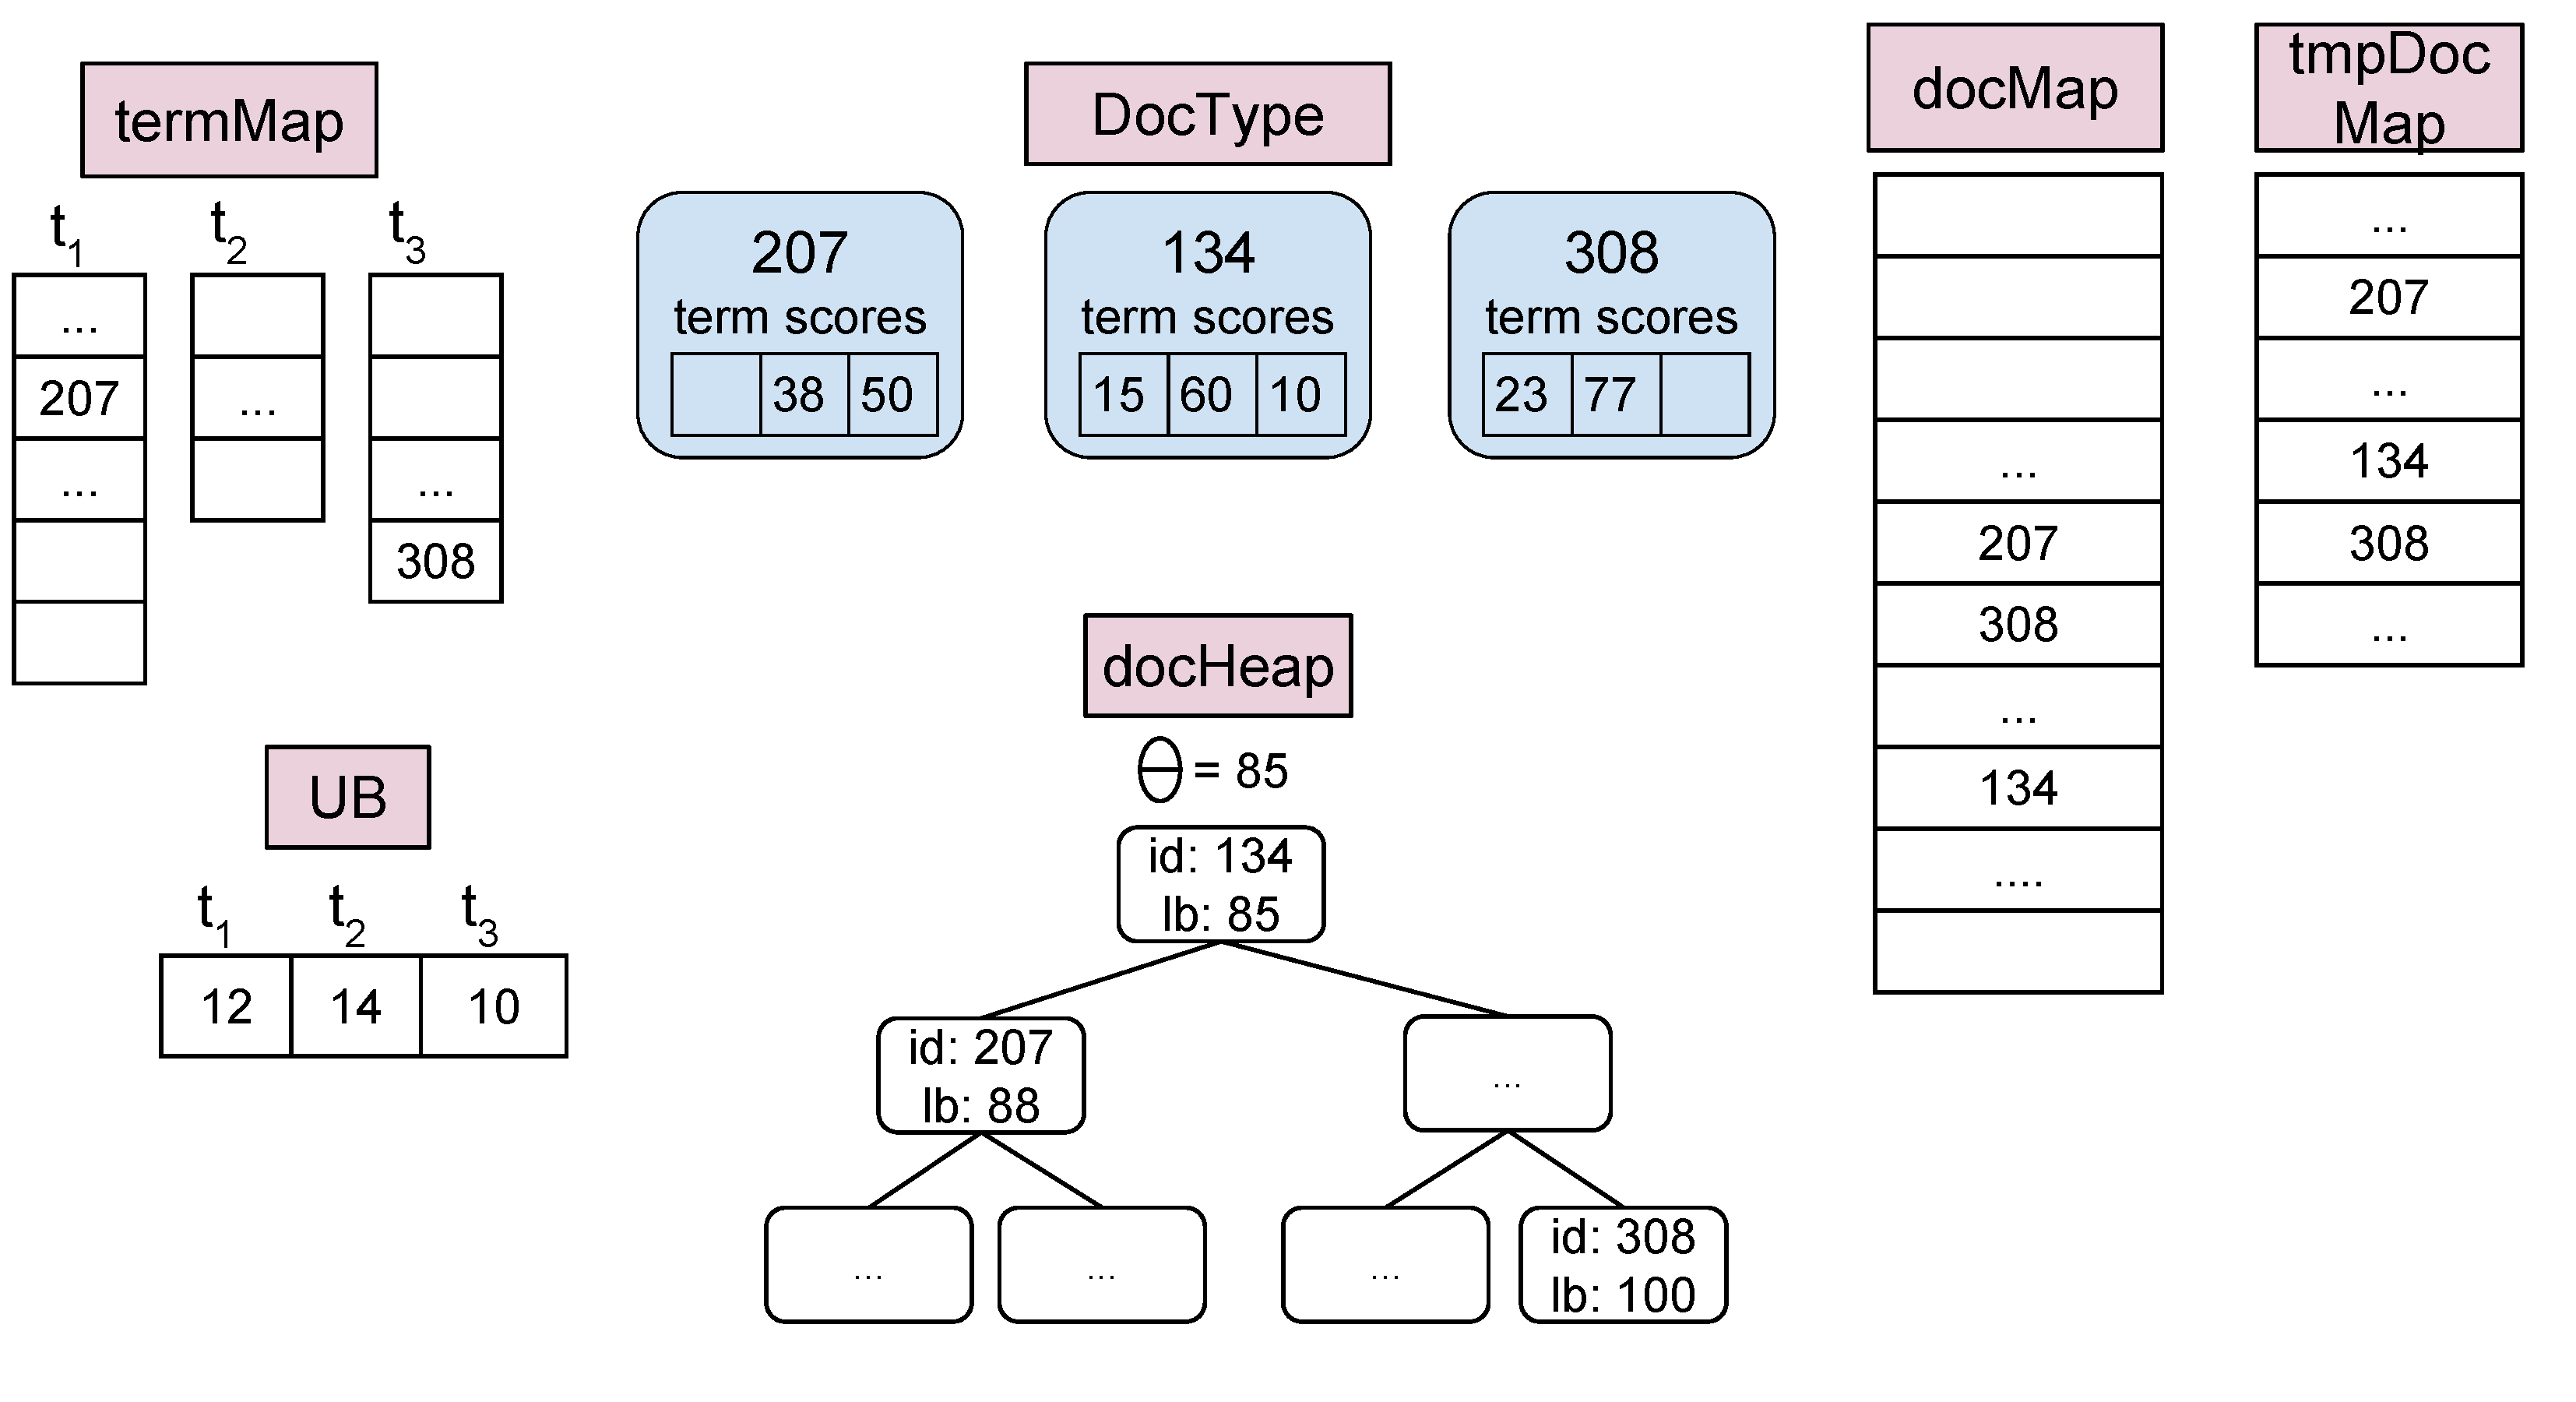
\includegraphics[width=0.7\columnwidth]{figures/localData}
\caption{\alg\/ data structures. The \DMap\ keeps track of partially scored documents; \LDMap\ and \TMap\ are local partial copies of \DMap.}
\label{fig:sparta_ds}
\end{figure}



\remove{

\begin{table*}[tb]
\centering
\begin{tabular}{l l l}
\hline
name & value & description\\
\hline
 \Docobj\ & $\langle$ int id, int score[$m$], int LB $\rangle$ & document object\\
 \DHeap & init empty &  heap of \Docobj\ sorted by LB \\
 $\Theta$ & init $0$  & minimal value in $\DHeap$\\
 $UB[m]$ & init $\infty$ & upper bounds on untraversed docs\\
 \RAStop&  $\sum_{i=1}^m UB[i] \le \Theta$ & UB stopping condition\\
 $UB(doc)$ & $\sum_{i=1}^m \big( doc.score[i] > 0$ $?$ $doc.score[i] : UB[i] \big)$ & document score upper bound \\
 \DMap & init empty & maps document id to \Docobj \\
 \HeapUpdateTime & init now & time of last heap update\\
 \Done & init false & termination indication\\
 \TMap[m] & init pointer to \DMap &  per-term partial copies of \DMap\\ 
  \LDMap & init empty & temporary \DMap\ for maintenance\\ 
  \hline
\end{tabular}
\caption{\alg's data structures and  initial values.}
\label{alg:sparta-ds}
\end{table*}

}

Table~\ref{alg:sparta-ds} defines the data structures used by \alg\
and Figure~\ref{fig:sparta_ds} illustrates them. 
As in NRA, the algorithm maintains the current top-k results in a heap, \DHeap, and its lowest value in $\Theta$. It keeps $m$ pointers to the next elements to traverse in all posting lists (not listed in Table~\ref{alg:sparta-ds})
and an array $UB$ of upper bounds on non-traversed term scores. 
$UB$ is used for computing the documents' upper bounds 
as well as for checking NRA's  stopping conditions.   

The hash map 
\DMap\ maps  document ids encountered thus far to document \Docobj\ objects. A \Docobj\ holds a vector of term scores observed thus far for this document as well as a lower bound on the document score computed as their sum.
%\DMap\ is used to maintain the partial document scores. 
NRA's first stopping condition is checked by the macro \RAStop, and the 
second stopping condition is checked as follows: 
\begin{equation} \label{eq:stop2}
\forall D\in \DMap \setminus \DHeap : UB(D) \le \Theta.
\end{equation}
The stopping conditions are evaluated by a \emph{cleaner} task,
which also checks the heap's latest update time \HeapUpdateTime\ and 
sets the \Done\ flag once the algorithm can stop.





In addition, to reduce the synchronization overhead and improve cache locality, \alg\ uses 
two local data structures that hold partial copies of the global \DMap, namely the \TMap\ array with a (local) hash map per term, 
and the \LDMap\ used by a dedicated maintenance thread. The role of these will become evident 
when we discuss synchronization and locality below.

\subsection{Splitting the Work}
\label{sssec:tasks}

%Executing NRA on a multi-term query sequentially can take a long time. We shorten this time by processing queries in multiple threads running in parallel. 

A na\"ive attempt to parallelize NRA would be to 
%assign a thread per term and 
share the data structures among all threads. (Note that sharing state is essential because the partial document scores, and consequently the lower bounds, are affected by multiple threads that generate term scores). This approach 
\remove{
suffers from multiple drawbacks. For one, it requires a predefined number of threads, while a server running many queries may not always have the required number of threads available. More importantly, straightforward sharing 
}
leads to high contention, primarily around $\DMap$.%, even when the implementation uses a state-of-the-art concurrent hash map\footnote{\small{\url{https://docs.oracle.com/javase/7/docs/api/java/util/concurrent/ConcurrentHashMap.html}}}. 
%This results in even poorer performance than the sequential execution.\inred{we need to justify it}
% (see Section~\ref{sec:eval}).   

%Instead, we redesign the algorithm flow in a way that reduces contention. 
To reduce contention, we 
consider the point in time when the first stopping condition (Equation~\ref{eq:stop}) holds. From this time on, no new document's score can surpass the lower bound of any document in the shared \DHeap. Therefore, adding new documents to \DMap\ is no longer helpful (a similar observation was made  in~\cite{Mamoulis:2007}). 
On the other hand, it is possible to shrink \DMap\ by removing documents whose upper bounds are smaller than $\Theta$.
This is cardinal for the concurrent implementation, which can stop sharing \DMap\ among the threads once it is sufficiently small, thereby eliminating the synchronization overhead. 




\begin{algorithm*}[htb]
\small
\begin{multicols}{2}
\begin{algorithmic}[1]
\For{$i=1$ to $m$} \Comment processing $m$-term query
\State add {\sc processTerm($i$)} to job queue \label{l:par-init-job}
%\State \TMap[i] $\leftarrow$ pointer to \DMap
\EndFor
\State spawn up to $m$ execution threads to run jobs from queue\label{l:start-threads}
\State wait until \RAStop
%\State	
	\Comment all candidate documents are in \DMap
\State add {\sc cleaner()} to job queue %\Comment parallel with term processing
\State wait until $done$
\State return \DHeap \label{l:par-end}
%

\Statex 
\Procedure{processTerm}{$i$} 
%\Statex
%	\State $\langle id,$ score$\rangle \leftarrow$ next entry in $i$th posting list
%  	\If{$id \not\in \DMap$}
%    	\State create new document object $D$
 %       \State add $D$ to $\DMap(id)$
%	\Else 
 %   	\State $D \leftarrow \DMap(id)$
%	\EndIf
%	\State {\sc evaluate}($D$, score, $i$)
 %   \State $UB[i] \leftarrow$ score 
  % 	\Comment update term's upper bound \label{l:seq-update-ub}
%\EndIf
%\Statex 
	\If{\RAStop\, $\wedge\, |\DMap | < \Phi $}  
		\Comment \DMap\ is shrinking and small
		\If{\TMap[i]=\DMap} \label{l:hash-start}
		\State {\sc initMap($i$)}
  	\EndIf \EndIf \label{l:hash-end}
%    \Statex
	\For{$j=1$ to \emph{segSize}} 
%	\Statex \Comment evaluate documents in segment
		\If{\emph{done}} return \EndIf
    		\State $\langle id,$ score$\rangle \leftarrow$ next entry in $i$th posting list
		\State $D \leftarrow$ \TMap$[i](id)$
 	  		\If{$D = \bot$} \Comment document missing 
 	  			\If{$\neg$\RAStop} \Comment hash incomplete
		 			\State create new document object $D$
 					\State add $D$ to $\TMap[i](id)$
				\Else\ continue
				\EndIf
    			\EndIf
        			\State $D.score[i] \leftarrow$ score \Comment update $D$'s term $t_i$ score
			\If{$\Sigma_{j=1}^{m} D.score[j] >  \Theta$}  
			\Comment $D$ belongs in heap
				\State {\sc update\_heap}($D$)
			\EndIf	
	\EndFor % $id$ is last in chunk
	\State $UB[i] \leftarrow$ score \Comment update term's upper bound \label{l:thread-update-ub}    
	\State add {\sc processTerm($i$)} to job queue \label{l:new-task}
\EndProcedure

%\Statex

\Procedure{initMap}{$i$}	
        			\Comment create cache-friendly local copy of \DMap\ %for evaluating term $i$
        			\State \TMap[i] $\leftarrow$ new hash map
    			\ForAll{$D \in$ \DMap\ where $D.score[i] = 0$} 
            			\State add $D$ to \TMap[i] \label{l:hash-chash}
            		\EndFor
\EndProcedure
\Statex 
\Procedure{update\_heap}{$D$} 
\State lock \DHeap \label{l:lock-heap}
\If{$D\not\in$\DHeap} 
	\State insert $D$ to \DHeap
	\ForAll{$d \in$ \DHeap}  \label{l:for-all-heap-docs}
		\State $d$.LB $\leftarrow \Sigma_{j=1}^{m} d.score[j]$
		\State move $d$ to correct place in heap \label{l:fix-heap}
	\EndFor
	\If{$|\DHeap | > k $} 
		\State remove doc with the lowest score from \DHeap
	\EndIf
	\If{$|\DHeap | = k $}
		\State  $\Theta \leftarrow$ lowest score in \DHeap
	\EndIf
	\State \emph{HeapUpdateTime} $\leftarrow$ current time 
\EndIf
\State unlock \DHeap  \label{l:unlock-heap}
\EndProcedure
%
%
\Statex 
\Procedure{cleaner}{} \label{l:clean-start}
%\While{\DMap\ has more than $k$ entries}
\If{$|\DMap | > \Phi $} 
\State \LDMap\ $\leftarrow$ new hash map \label{l:clean-local-copy}
%a local copy of \DMap 
\For{every doc $D$ $\in$ \DMap} 
\If{$UB(D) > \Theta \vee D \in$ \DHeap}
	\State add   $D$ to \LDMap
\EndIf
\EndFor
\State replace \DMap\ by \LDMap \label{l:clean-replace}
\EndIf
%\Statex
%\State \emph{Stop} $\leftarrow \big( |\DMap| = |\DHeap| \big)$ 
\If{\emph{HeapUpdateTime} $ + \Delta < $ now $\vee\ \big( |\DMap| = |\DHeap| \big)$ } \label{l:clean-stop-cond}
\State \emph{done} $\leftarrow$ true
\Else\ add {\sc cleaner()} to job queue
\EndIf
\label{l:clean-end}
%\EndWhile
\EndProcedure 
\end{algorithmic}
\end{multicols}
\caption{\alg\ algorithm.}
\label{alg:sparta}
\end{algorithm*}

\alg's pseudocode appears in Algorithm~\ref{alg:sparta}. It 
exploits up to $m$ {\em worker\/} threads per query, but can run with fewer threads if less are available. 
We divide posting list traversals to segments of size \emph{segSize}, and use a job queue to allocate posting list segments to threads (line \ref{l:par-init-job}). 
The  {\sc processTerm($i$)} function processes the next segment of term $t_i$. 
A  thread that finishes its assigned segment inserts into the queue a new task for scanning the next segment in the same term's posting list 
(line~\ref{l:new-task}). Thus, we  progress on all posting lists at the same rate modulo the segment size. 
In case $m$ threads are available, a large segment size can be used.

In addition to  posting list-traversing tasks, the 
{\sc cleaner} function (lines~\ref{l:clean-start}--~\ref{l:clean-end}) performs maintenance on the \DMap.
This task is invoked once Equation~\ref{eq:stop} holds and so  \DMap\ no longer grows.
The cleaner serves two purposes. First, as its name suggests, it removes 
entries that ceased to be top-k candidates from \DMap. %, thus reducing its size.  
Since \alg\ is memory-intensive, a smaller \DMap\  allows it to run much faster; 
(a similar observation, in a sequential setting, was made in~\cite{Gursky:2008}). 
Second, it detects the stopping conditions (line \ref{l:clean-stop-cond}). In the approximate version, it checks whether the heap has not changed for $\Delta$ time 
(the exact version is obtained by setting $\Delta=\infty$). It also checks the  condition of Equation~\ref{eq:stop2}: 
once \DMap\ is the same size as \DHeap\ we know that the two are identical because \DMap\ always includes all \DHeap\ entries. 
At this point, \DHeap\ holds the top-k scored results, and stopping is safe. 
%
Once the algorithm stops, the main thread returns the heap's contents. 

\subsection{Synchronization} 
\label{sec:synch}

Note that, \DHeap, $UB$, \DMap, and \Docobj\ objects referenced by them are accessed concurrently by multiple threads. We need to protect such access to avoid inconsistencies. On the other hand, reducing contention is crucial for performance. Moreover, 
\alg\ is a memory-intensive algorithm, and 
%primarily with respect to the shared \DMap. During the parallel phase, multiple threads access it frequently, for reading. 
in order to keep the memory access latencies low, it is paramount to exploit the CPU hardware cache, in particular the core-private L1 caches. 
We now explain how we synchronize access to each of the shared variables
in a way that reduces contention and improves cache utilization. 



Since at most one thread processes each term, no races arise around updating $UB$ entries, and no lock is needed. However, 
all threads read all $UB$ entries, and therefore frequent updates can lead to frequent cache misses, and in turn, poor performance. 
%Note that during the sequential phase, the UB array is updated after each partial document evaluation (line \ref{l:seq-update-ub}), which occurs frequently.
In order to reduce the number of cache misses, instead of updating $UB$ after each document evaluation, the workers update it lazily, at the end of a segment traversal (line \ref{l:thread-update-ub}). Since upper bounds can only decrease whereas $\Theta$ can only increase, such lazy updates do not affect correctness.

%while speeding up the execution.
Updates of \DHeap\ and $\Theta$ are protected by a shared lock (lines~\ref{l:lock-heap} and~\ref{l:unlock-heap}), which  serializes all updates. 
%However, since most heap updates occur in the sequential phase, parallel updates are infrequent, and this does not constitute a performance bottleneck. 
To avoid races around evaluating a \Docobj's
lower bound and inserting it into \DHeap, we update the lower bound in a lazy manner while holding the global lock on \DHeap: Every thread that adds a document to the heap updates the lower bounds of all heap documents (lines \ref{l:for-all-heap-docs}-\ref{l:fix-heap}).

Before the first stopping condition (Equation~\ref{eq:stop}) holds, multiple workers update \DMap\/ concurrently. 
We therefore protected each hash bucket by a granular lock, which  
performed better than the generic Java concurrent hashmap~\cite{java-hashmap}.


The cleaner task starts removing elements from  \DMap\/ after it is guaranteed that 
no new entries are added to  it; such removals substantially improve the term processing performance. 
Nevertheless, allowing the cleaner to constantly update \DMap\ would lead to frequent cache invalidations at the
tasks that read the map. 
To avoid frequent cache misses, 
%such frequent synchronization between the cleaner and term-processing tasks, 
the global map is kept read-only most of the time, while the cleaner works on a local copy: 
it  
%Specifically, as long as its stopping condition is not satisfied, 
%the cleaner 
repeatedly builds a new map \LDMap, holding \DMap\ entries whose upper bounds 
are higher than $\Theta$ as well as ones that are included in \DHeap\ (whose upper bounds may be exactly $\Theta$); recall that other \DMap\ entries no longer need to be kept. 
Once \LDMap\ is ready, the cleaner replaces \DMap\ with it via a single pointer swing 
(flipping the global reference). 

%\subsection{Locality Optimizations}
%\label{sssec:locality}

%\alg\/ is a memory-intensive algorithm, primarily with respect to the shared \DMap. During the parallel phase, multiple threads access it frequently, for reading. In order to keep the memory access latencies low, it is paramount to exploit the CPU hardware cache, in particular the core-private L1 caches. 

%We call this concurrent algorithm SharedState. SharedState runs much faster than the sequential NRA, and scales to very long queries. We now proceed to the full version of \alg, which further improves the performance. \inred{Gali: the full version only adds the local hash maps, so maybe we should present it in a different way. We also don't have to present SharedState here, it can be done in the evaluation section}

Access to \DMap\ is a principal performance bottleneck, since it is frequently read by all worker threads. Initially, it is too large to fit into local caches, and so the parallel execution inherently requires global memory accesses. But thanks to the cleaner's work, \DMap\ shrinks in the course of the execution. 
Moreover, not all  \DMap\ entries are relevant for all terms -- if $D$'s term score for $t_i$ has already been computed, then a  thread handling term $t_i$ does not need to access $D$.
Thus, the relevant subset of  \DMap\ for each term eventually becomes small enough to fit in its local cache. As long as the thread continues to access the global \DMap,  it  experiences massive cache misses every time the cleaner replaces the global \DMap. 
%As long as $\DMap$ is big, it is more important to shrink it fast than avoid those misses. However, 
But 
once it becomes small enough to fully fit in the local cache, there is no need to keep using the global copy. 

To this end, \alg\/ associates a local map replica, \TMap, with each posting list. \TMap\ is created by the worker that currently owns that posting list once \DMap's size drops below a threshold $\Phi$,
in our implementation, $\Phi=10$K entries. The {\sc initMap} function scans \DMap, and copies to \TMap\ the references to those \Docobj{} objects that do not contain the score for the worker's term yet.  Once a \TMap\ has been created, every worker that handles its posting list uses it.
Note that since every posting list is accessed by a single worker at any given time, no synchronization is required.
%
%We show in the next section that by using \TMap s, we expedite \alg's query processing latency by up to $35\%$.

\subsection{Analysis}
\label{ssec:analysis}

\alg\ accesses posting lists in the same manner as NRA does, and stops only when NRA's stopping conditions hold. Thus, like NRA, its 
exact version ($\Delta = \infty$) is safe, and returns the top-k results. 

In terms of performance, NRA was shown to be \emph{instance-optimal} when  random access is impossible~\cite{Fagin:2001}, 
namely, its number of accesses to posting list entries is asymptotically close the optimum for every problem instance.  
This property holds for pNRA as long as the rates in which different threads access different posting lists are within constant multiples of each other~\cite{Fagin:2001}, because in this case a thread that ``runs ahead'' without knowing it should stop only accesses a constant factor more entries than the algorithm needs to, which the asymptotic
analysis ignores. \alg\ differs from pNRA in deferring updates to UB until the end of the segment, 
which may further delay stopping for \emph{segSize} additional posting list accesses. Since \emph{segSize} is constant, \alg\ is asymptotically
instance-optimal under the same assumptions as pNRA.


